\section*{Original Section 4.2.3: Directing the Flow (pp.17:14--18)}
Let us remind that we deal with $\varphi:=\Flow_G^{\eta^{k_0+1}}$. To show that there is a path consistent with $\zeta$ from $v_{k_0+1}$ to a leaf with a label $C\in\mathcal C$ we show that $(\varphi\setminus\mathcal C)|_\zeta$ is satisfiable and hence there should be an extension of $\zeta$ that violates only clauses from $\mathcal C$.
\begin{result}{Remark 21}
If we do not care about assignment $\zeta$, the statement is trivial, since $\varphi$ is so-called minimally unsatisfiable formula (that becomes satisfiable after removing any clause). But $\zeta$ transforms our formula to ``heavily unsatisfiable'' formula, since $\zeta$ $0.6$-satisfies a lot of vertices (that was the crucial property that we used to create a garland).
\end{result}
Note that by construction of $\eta^{k_0+1}$ for each $v\in V$ there exists a clause $D\in\mathcal D$ that had originated from the constraint for $v$. For each $v$, we pick any such clause and denote it by $D_v$. We divide the rest of the proof into two parts.
\begin{enumerate}
\item ``Local part''. We find a carefully chosen large enough set of vertices $U\in V$ and an assignment $\tau\supseteq\zeta$ such that there is a set $V_\tau\supseteq(U\cup V_\zeta)$:
\begin{itemize}\item $(V\setminus V_\tau,E\setminus\supp(\tau))$ satisfies $(r,\beta')$-expansion property;
\item for all $v\in U$ the assignment $\tau$ violates $D_v$ and hence $\tau$ assigns all edges incident to $v$;
\item for all $v\in V_\tau\setminus U$ the assignment $\tau$ satisfies constraint for $v$.\end{itemize}
For this part we use the simplified version of technique used for the garland creation.
\item ``Global part''. By using Max-Flow Min-Cut Theorem we show that $\tau$ can be extended to total assignment that satisfies constraints for vertices whose constraints are neither satisfied nor falsified by $\tau$ yet.
\end{enumerate}
Since we satisfy all the constraints of $(\Flow_G\setminus\mathcal D)_\zeta$ this assignment also satisfies all constraints in $(\varphi\setminus\mathcal C)|_\zeta$ by the construction of the formula $\varphi$ (clauses of $\varphi$ are the weakened versions of the clauses $\Flow_G$).
Before we proceed with the proof let us define the ``overflow''.
\begin{result}{Definition 22}
The overflow introduced by a locally consistent assignment $\sigma$ is:
\[\of_\sigma:=1+\sum_{v\in V_\sigma}\left(\sum_{e\in E:\st(e)=v}x_e-\sum_{e\in E:\en(e)=v}x_e-c(v)\right).\]
\end{result}
Note that $\of_\zeta\le|\zeta|+1\le\nu_{k-1}\Delta r+1$.
\subsection*{4.2.3.1 Local part}
We start with the local part of the proof. In the beginning of our construction $U_0:=\emptyset$, $\tau_0:=\zeta$, $V_{\tau_0}:=V_\zeta$ and $i:=0$.
We repeat the following process while $\of_{\tau_i}>0$.
\begin{enumerate}
\item Choose a vertex $u_i$ that is untouched by $\tau_i$.
\item Let $\rho_{u_i}$ be an assignment to edges that are incident to $u_i$ such that $D_{u_i}$ is unsatisfied by $\rho_{u_i}$.
\item $\tau':=\tau_i\cup\rho_{u_i}$. Since $u_i$ is untouched by $\tau_i$ there is no intersection between $\rho_{u_i}$ and $\tau_i$.
\item Let $H_i\subseteq V\setminus V_{\tau_i}$ be the maximal set of vertices that satisfies:
\[|H_i|\le r;\qquad |E(H_i,\overline{H_i}\setminus\{u_i\})\setminus\supp(\tau_i)|\le\beta'\Delta|H_i|.\]
Let $\kappa_i$ be an assignment on variables that correspond to edges in the set $E(H)\setminus\supp(\tau')$ such that for all $v\in H_i$:
\[\sum_{e\in E:\st(e)=v}(\tau'\cup\kappa_i)(x_e)-\sum_{e\in E:\en(e)=v}(\tau'\cup\kappa_i)(x_e)=c(v).\]
\item $U_{i+1}:=U_i\cup\{u_i\}$, $\tau_{i+1}:=\tau'\cup\kappa_i$ and $V_{\tau_{i+1}}:=V_{\tau_i}\cup H_i\cup\{u_i\}$.
\item $i:=i+1$.
\end{enumerate}
Let $\ell$ be a number of iterations in this process. Let $U:=U_\ell$ and $\tau:=\tau_\ell$.
At first we give an upper bound on $\ell$. Since for all $i$ an assignment $\kappa_i$ exactly satisfies vertices in $H$, inclusion of $H$ into $V_\tau$ does not change the overflow. Assignment $\rho_{u_i}$ violates $D_{u_i}\in\mathcal D$ and by definition of $\eta^{k_0+1}$:
\[-\frac\Delta4-1\le\sum_{e\in E:\st(e)=u_i}\rho_{u_i}(x_e)-\sum_{e\in E:\en(e)=u_i}\rho_{u_i}(x_e)\le-\frac\Delta4.\]
Hence on each iteration $\of_{\tau_{i+1}}\le\of_{\tau_i}-\Delta/4$ and $|U|\le4|\zeta|/\Delta$ and $-\Delta/4-1\le\of_\tau\le0$.
\begin{result}{Lemma 23}
For all $i\le\ell$:
\begin{itemize}\item $\kappa_i$ exists;
\item $|V_{\tau_i}|\le\frac{1}{(\beta-\beta')\Delta}(\supp(\zeta)+\Delta|U_i|)$ and hence $|\tau_i|\le\frac{2}{\beta-\beta'}(|\supp(\zeta)|+\Delta|U_i|)$;
\item $(V\setminus V_{\tau_i},E\setminus\supp(\tau_i))$ satisfies $(r,\beta')$-expansion property.\end{itemize}
\end{result}
\begin{proof}This Lemma may be considered as simplified version of Lemma 18. For the proof see Appendix A.\end{proof}
To conclude the construction note that $\tau_i\le\tfrac{10}{4}\nu_{k-2}\Delta r\le\tfrac\Delta4 r$ for all $i\le\ell$ and we always can find the vertex untouched by $\tau_i$.
\begin{result}{Remark 24}This is the only place where we use that $r\le n/\Delta$.\end{result}
\subsection*{4.2.3.2 Global part}
Let $B:=V_\tau\setminus V_\zeta$. For the vertex $v\in V$ the overflow of $v$ is defined in the following way:
\[\of(v):=-\sum_{\substack{e\in\supp(\tau)\\\st(e)=u}}\tau(x_e)+\sum_{\substack{e\in\supp(\tau)\\\en(e)=u}}\tau(x_e)+c(v).\]
We want to create an auxiliary graph. Let $F^+:=\{v\in V\setminus V_\tau\mid\of(v)>0\}$ and $F^-:=\{v\in V\setminus V_\tau\mid\of(v)<0\}$. See Fig.2.
We define a graph $G':=(V',E')$ on vertices $V':=(V\setminus V_\tau)\cup\{s\}\cup\{t\}$, where $s$ is a source and $t$ is a sink. Edges $E'$ include four groups:
\begin{center}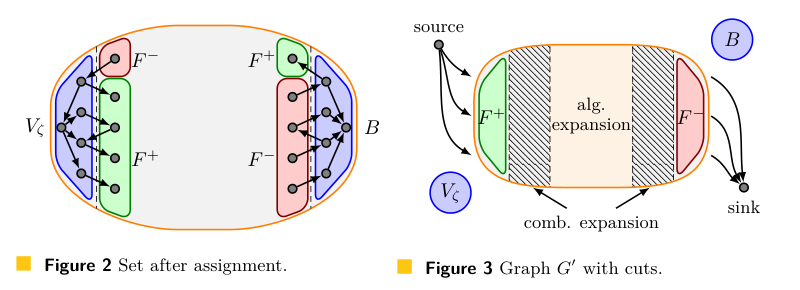
\includegraphics[width=.95\linewidth]{fig23.png}\end{center}
\begin{itemize}\item $E\setminus\supp(\tau)$;
\item we connect $s$ with all $v\in F^+$ by $\of(v)$ number of edges;
\item we connect $t$ with all $v\in F^-$ by $-\of(v)$ number of edges;
\item if $\of_\tau<0$ we choose an arbitrary set of vertices $S\in V\setminus V_\tau$ of size $|\of_\tau|$ and connect all $v\in S$ with $s$ by one more edge.\end{itemize}
See Fig.3.
\begin{result}{Remark 25}
\begin{enumerate}\item $\deg(s)=\deg(t)$;
\item If $A\subseteq V'$ then $E(\{s\},A)\le\Delta/4+1+\sum_{v\in A}\of(v)$ and $E(\{t\},A)=-\sum_{v\in A}\of(v)$.\end{enumerate}
\end{result}
\begin{proof}The first property follows from the construction of $\tau$ and the second one follows from definition of $G'$.\end{proof}
Let $f:=\deg(s)$. To conclude the proof we want to show that there is an $s$-$t$ flow in $G'$ of size $f$ (assuming that capacity of each edge is $1$) and that if this flow exists, then we have an extension of $\tau$ that satisfies $\Flow_G\setminus\mathcal D$. As we mention above together these facts imply that $(\Flow_G\setminus\mathcal D)|_\tau$ is satisfiable hence $(\Flow_G\setminus\mathcal D)|_\zeta$ is satisfiable and $(\varphi\setminus\mathcal C)|_\zeta$ is also satisfiable hence there is a path from $v_{k_0+1}$ to a leaf marked by some $C\in\mathcal C$ which is a contradiction with an existence of a garland and an assumption about size of the branching program.
We start with the second part. Suppose that we have a flow of size $f$. Fix the flow that achieves this value. We define a total proper assignment $\sigma\supseteq\tau$ in the natural way. Consider an edge $e\in E'\cup E$ and $a=(u,v)$, $a'=(v,u)$ its directed copies. If there is a flow on the edge $e$:
\begin{itemize}\item from $u$ to $v$ then $x_a=1$ and $x_{a'}=0$;
\item from $v$ to $u$ then $x_a=0$ and $x_{a'}=1$.\end{itemize}
otherwise we set $x_a=0$ and $x_{a'}=0$.
Note that $f=\deg(s)$ hence we use all edges that connect $s$ with other vertices to push the flow. That implies for all $v\in V\setminus V_\tau$:
\[\sum_{\substack{e\in\supp(\sigma)\setminus\supp(\tau)\\\st(e)=v}}\sigma(x_e)+\sum_{\substack{e\in\supp(\sigma)\setminus\supp(\tau)\\\en(e)=v}}\sigma(x_e)=|E(s,v)|=\of(v)\]
and hence
\[\sum_{e\in E:\st(e)=v}\sigma(x_e)+\sum_{e\in E:\en(e)=v}\sigma(x_e)=c(v).\]
and constraints for all vertices in $V\setminus V_\tau$ are satisfied, but $\tau$ itself satisfied all constraints in $\Flow_G\setminus\mathcal D$ that correspond to vertices in $V_\tau$. Altogether it says that $\sigma$ satisfies all constraints in $\Flow_G\setminus\mathcal D$ as desired.
It remains to show that we have an $s$-$t$ flow of size $f$ in $G'$. To do it we use the Max-Flow Min-Cut Theorem and show that minimal $s$-$t$ cut has size $f$. Consider such a cut $(S,T)$, where $S,T$ are disjoint subsets of $V'$ such that $s\in S$ and $t\in T$. We consider two cases:
\begin{itemize}\item either $S$ or $T$ is small enough, then we use the $(r,\beta')$-expansion property that we have after removing $\supp(\tau)$ and $V_\tau$ from $G$;
\item $S$ and $T$ are large enough, then we use the Mixing Lemma to show that even removing $\supp(\tau)$ from $G$ cannot destroy balanced cuts.\end{itemize}
see Fig.3.
\begin{center}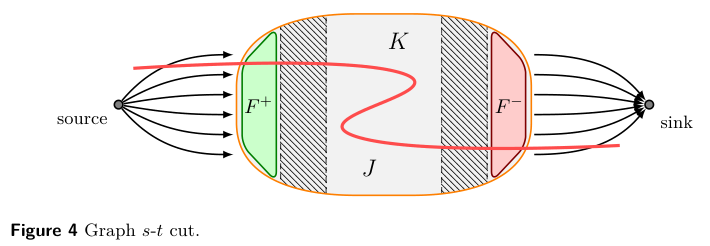
\includegraphics[width=.8\linewidth]{fig4.png}\end{center}
Consider an arbitrary $s$-$t$ cut $S\cup T$. Let $J:=S\setminus\{s\}$ and $K:=T\setminus\{t\}$ (see Fig.4). Consider the following cases.
\begin{enumerate}
\item If $J=\emptyset$ or $K=\emptyset$ then size of $(S,T)$ cut equals $\deg(s)$ or $\deg(t)$ respectively and we are done.
\item $0<|J|\le r$ or $0<|K|\le r$. Wlog assume that $|J|\le r$. Note that:
\[E_{G'}(S,T)=E_{G'}(\{s\},K)+E_{G'}(\{t\},J)+E_{G'}(J,K).\]
$E_{G'}(\{s\},K)=\sum_{v\in F^+\cap K}\of(v)$, so by Remark 25 to give a lower bound on the size of cut it is enough to show that $E_{G'}(J,K)\ge\Delta/4+1+\sum_{v\in F^+\cap J}\of(v)$. But $(V\setminus V_\tau,E\setminus\supp(\tau))$ satisfies $(r,\beta')$-expansion property. Hence
\begin{itemize}\item for all $v\in V\setminus V_\tau$: $|\of(v)|\le0.1\cdot\Delta$;
\item $|E_{G'}(J,K)|\ge0.9\cdot\Delta|J|$,\end{itemize}
that implies that $|E_{G'}(J,K)|-\Delta/4-1\ge2\sum_{v\in F^+\cap J}\of(v)$.
\item $|J|>r$, $|K|>r$. Wlog assume that $|J|\le|K|$. By Mixing Lemma:
\begin{align*}
|E_G(J,\overline J)|&=\Delta|J|-E_G(J,J)\ge\Delta|J|-\frac\Delta n|J|^2-\alpha\Delta|J|\\
&\ge\Delta|J|-|J|-\alpha\Delta|J|\ge0.9\cdot\Delta r,
\end{align*}
and
\[|E_{G'}(J,K)|\ge|E_G(J,\overline J)|-|\supp(\tau)|\ge0.6\cdot\Delta r.\]
On the other hand:
\begin{align*}
f&=\sum_{v\in F^+}\of(v)\\
&=\sum_{v\in F^+}\left(-\sum_{\substack{e\in\supp(\tau)\\\st(e)=u}}\tau(x_e)+\sum_{\substack{e\in\supp(\tau)\\\en(e)=u}}\tau(x_e)+c(v)\right)\\
&\le|\supp(\tau)|\le\frac\Delta4 r.
\end{align*}
\end{enumerate}
Hence in all cases $(S,T)$ has size at least $f$ which by Max-Flow Min-Cut Theorem implies the existence of flow in $G'$ of size at least $f$. That as mentioned above implies the desired lower bound on the size of branching program.
